\newpage
\section{CNN for Darcy equation}
\begin{breakablealgorithm}
	\caption{$u={\rm DarcyCNN}(\kappa; f_d, coarse\_grid\_size,)$}
	\label{alg:mgnet}
	\begin{algorithmic}
		\State Initialization:  $\kappa$
		%		\State Initialization $u^{1,0}$
%		\For{$ = 1:N_{epoch}$}
%		\For{$i = 1:\nu_$}
		\State Encode
		\begin{equation}
		u^{} = K^{3}  \ast_2 \sigma \circ K^{ 2}\ast \sigma (K^{ 1}\ast \kappa).
		\end{equation}
	
%		\EndFor
		\State Restriction to the coarse grid
		\begin{equation}
		u^{} = \sigma \circ \theta^{. 1} \circ u^{}
		\end{equation}
		\State
		Convolution on the coarse grid
		\begin{equation}
		u^{} =  \sigma \circ K^{ 5}\ast \sigma (K^{ 4}\ast u^{}).
		\end{equation}
		\State Decode
		\begin{equation}
		u^{} =  \sigma \circ \theta^{ 3}\circ \sigma (\theta^{ 2}\circ u^{}).
		\end{equation}
%		\EndFor
	\end{algorithmic}
\end{breakablealgorithm}

	where $K^{3}  \ast_2$ is the average pooling with kernel size $2  \times 2$ and stride 2, $K^{1}$, $K^{2} $, $K^{4} $ and $K^{5}  $ are multi-channel kernels with kernel size $3  \times 3$ and the size of these kernel matrices are $(1 \times f_d/2)$, $ (f_d/2 \times f_d)$, $(1,f_d/2)$ and $(f_d/2, f_d)$ respectively.
	
The loss function is 
$$
L = \frac{1}{N} \sum_{i=1}^{N} \frac{\| u_{pred} - u_{test}\|_{L^2}^2}{\| u_{test}\|_{L^2}^2}
$$

For this problem, we have a comparison for the results with and without nonlinear activation functon.
\begin{figure}[H]
	\centering
	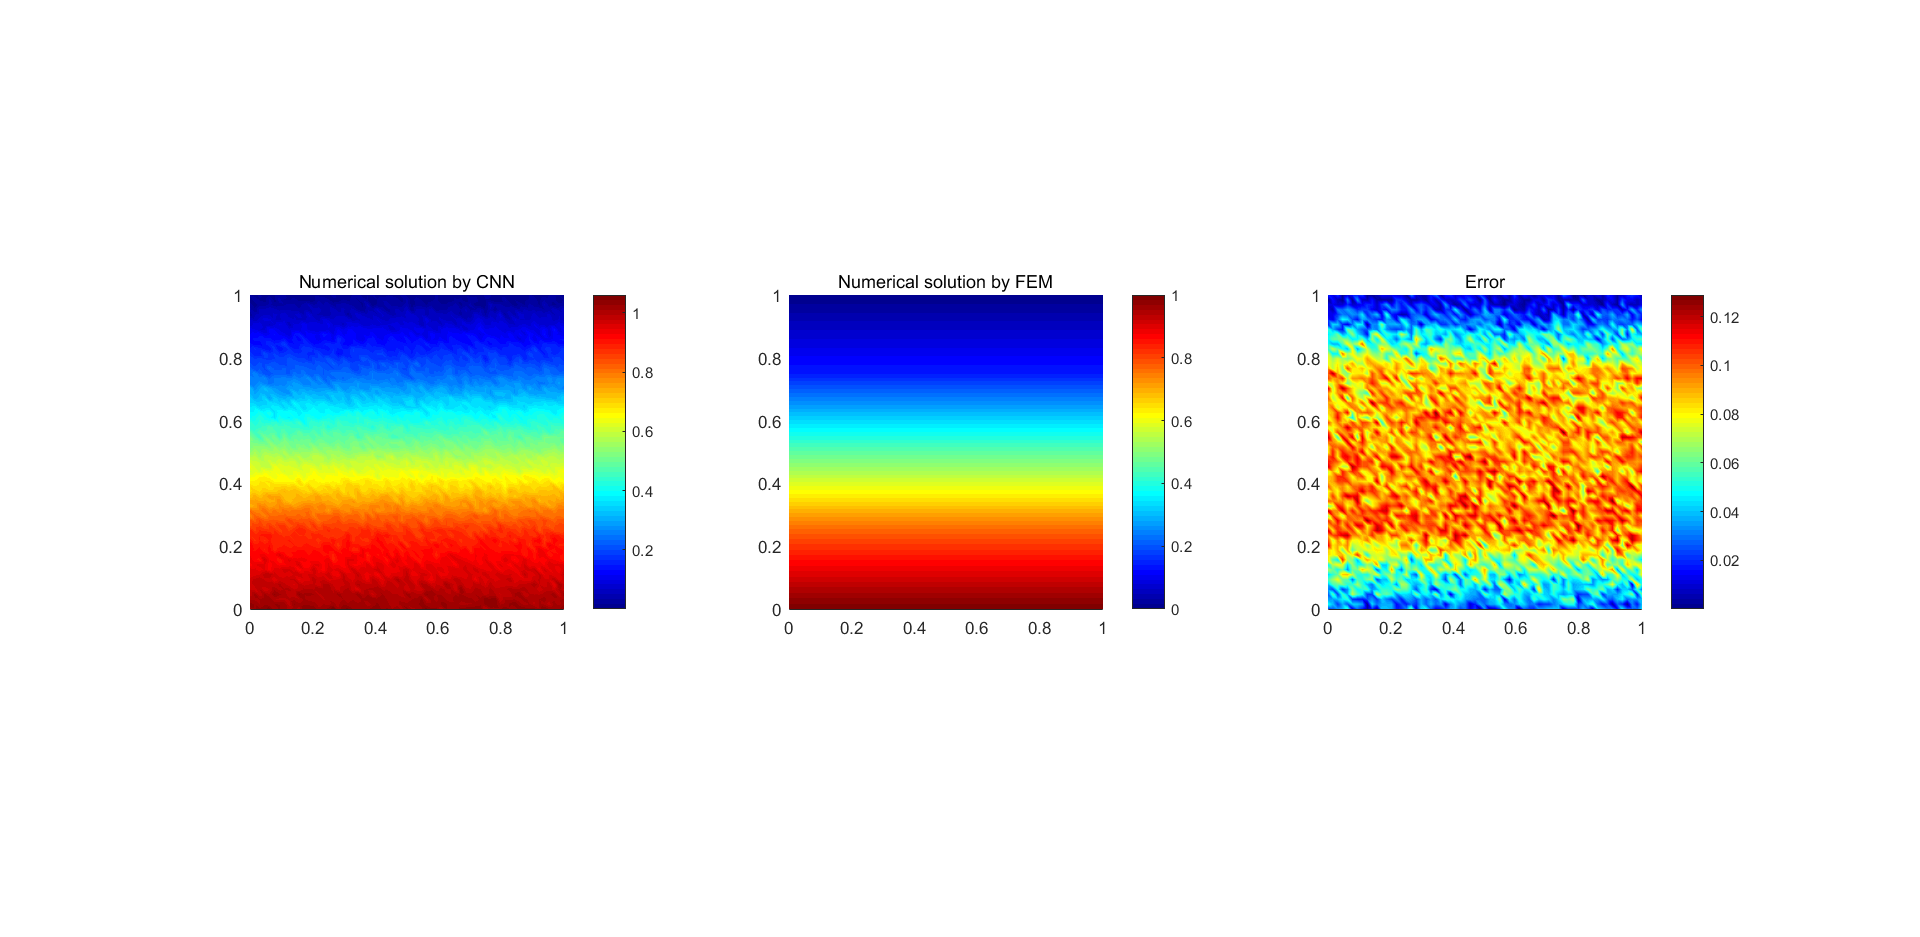
\includegraphics[width=0.65\textwidth]{figures/Darcy_CNN/Darcy_CNN_2000.png}
	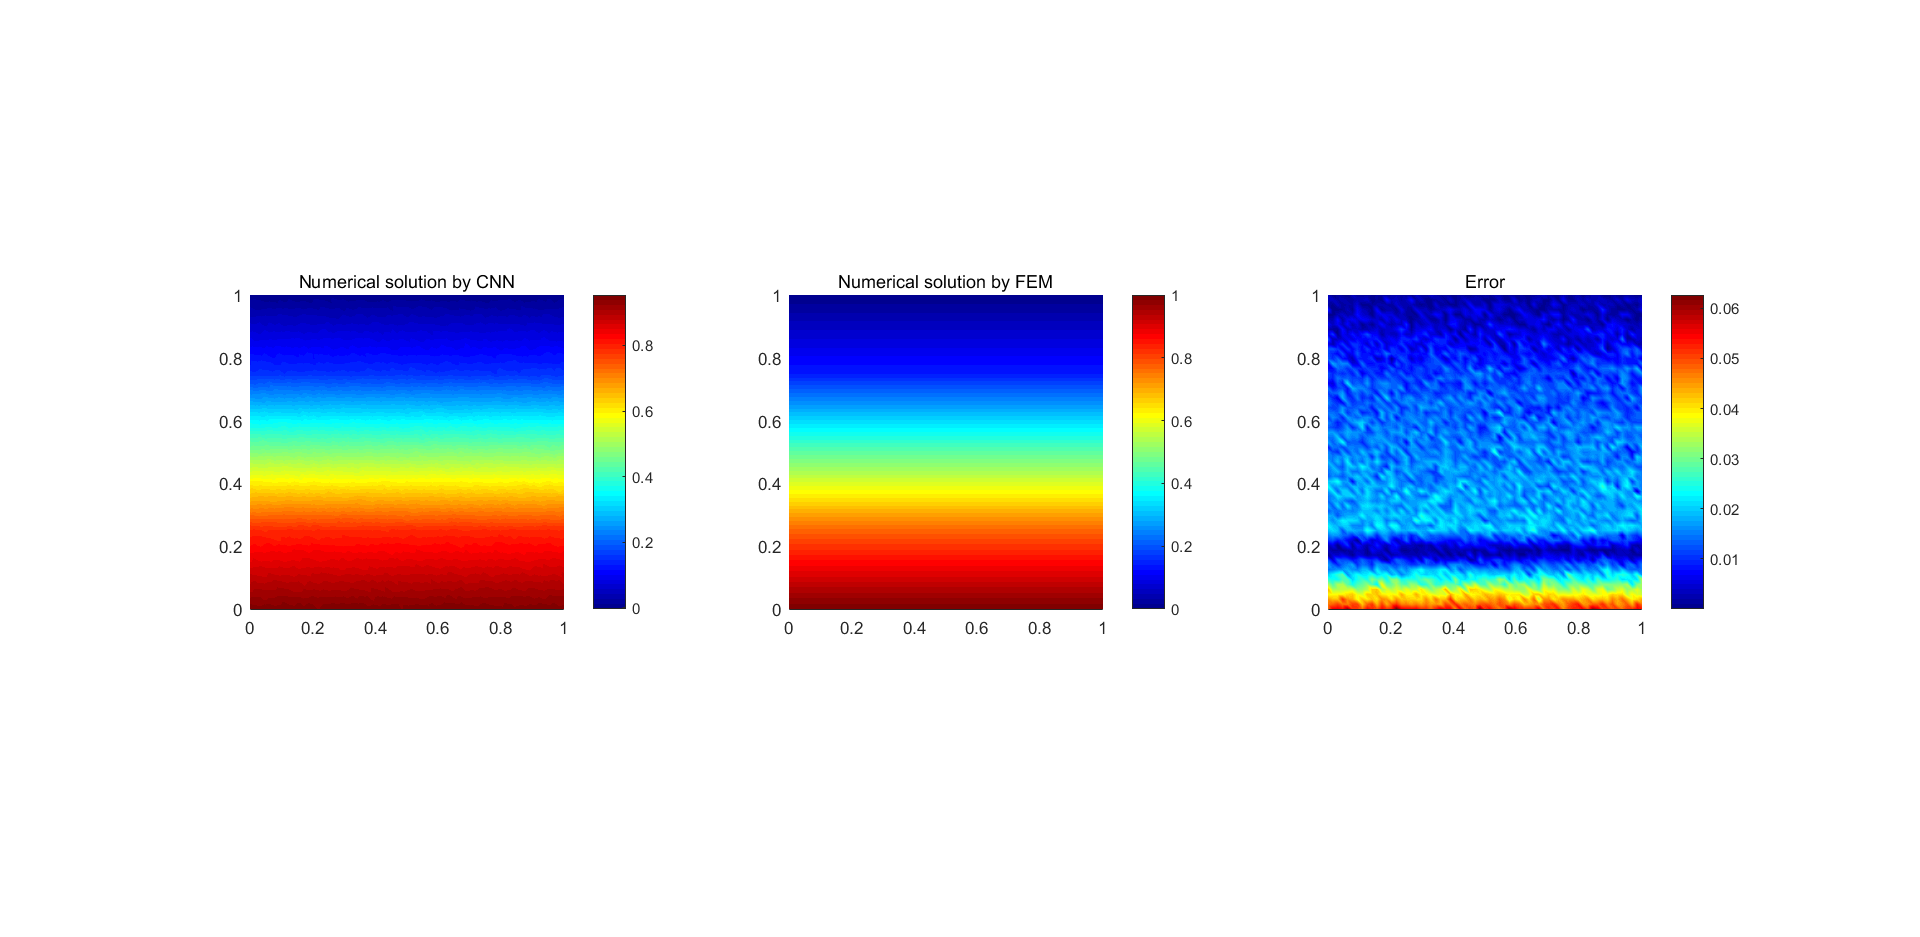
\includegraphics[width=0.65\textwidth]{figures/Darcy_CNN/Darcy_CNN_2000_nonlinear.png}
	\caption{Comparison of the solutions obtained by CNN with and without activation function by SGD (Top: without activation, Bottom:  with activation, 8,2 million parameters).}
\end{figure}

\begin{figure}[!htbp]
	\centering
	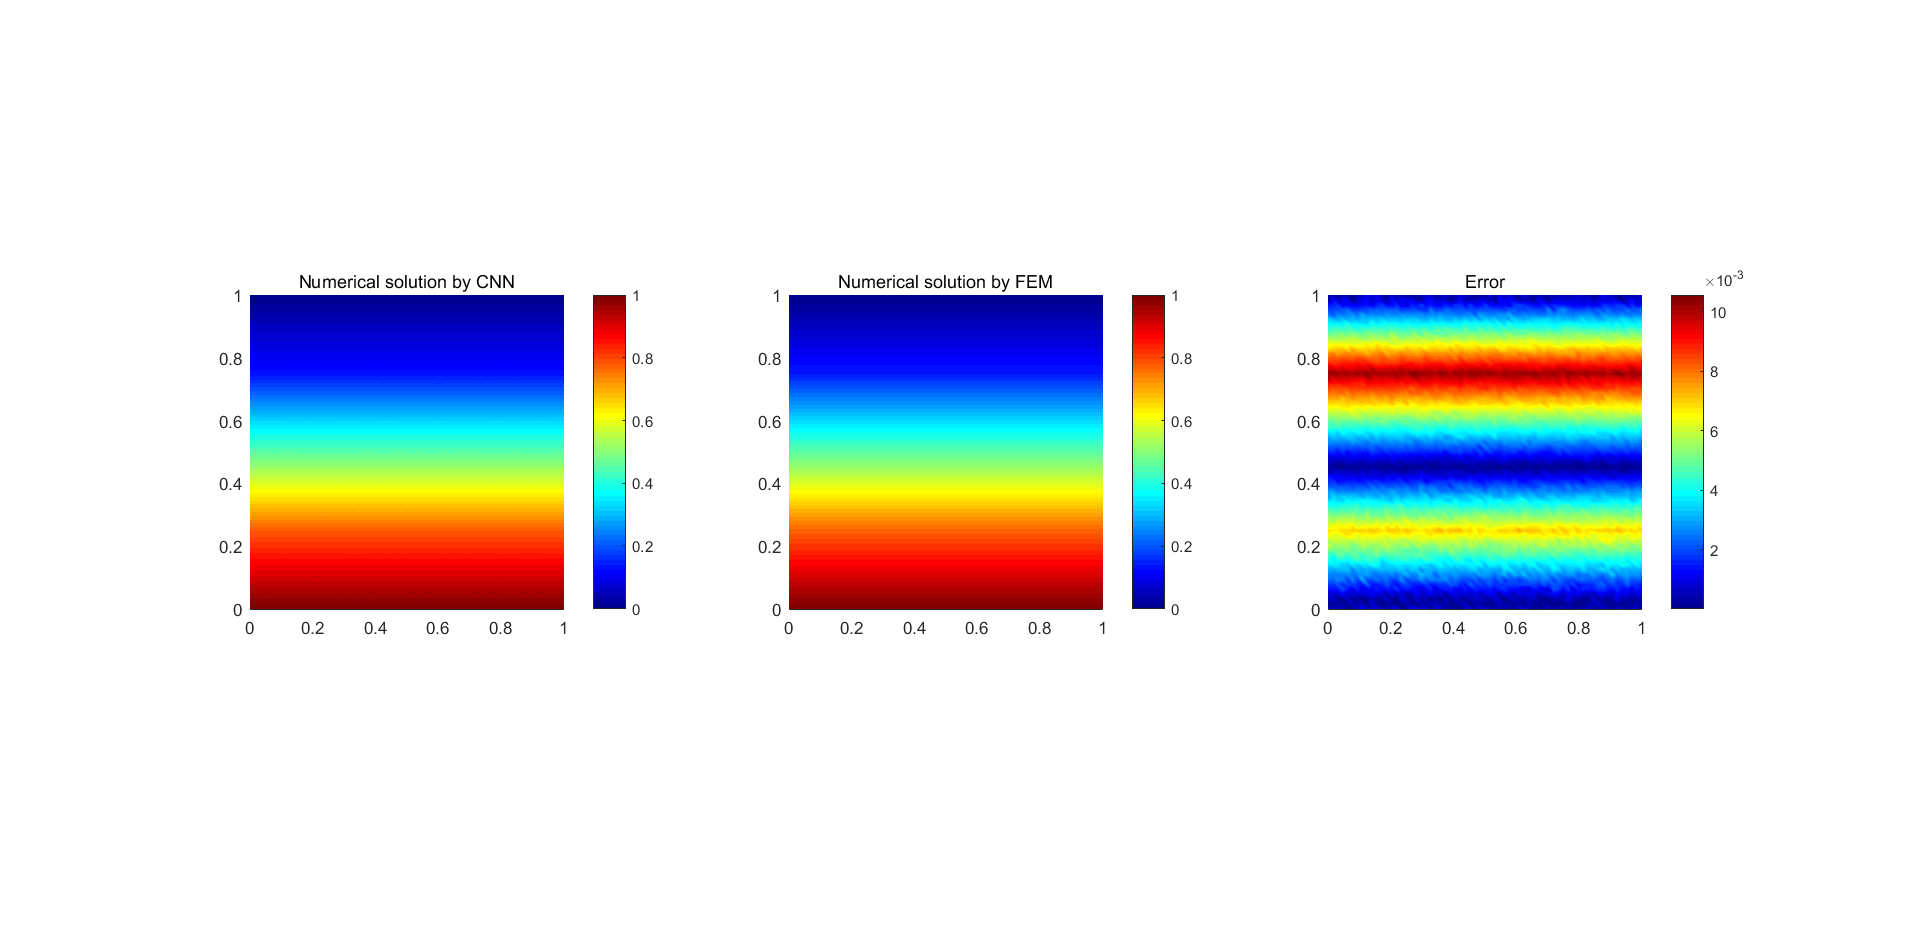
\includegraphics[width=0.65\textwidth]{figures/Darcy_CNN/Darcy_CNN_Adam_2000.png}
	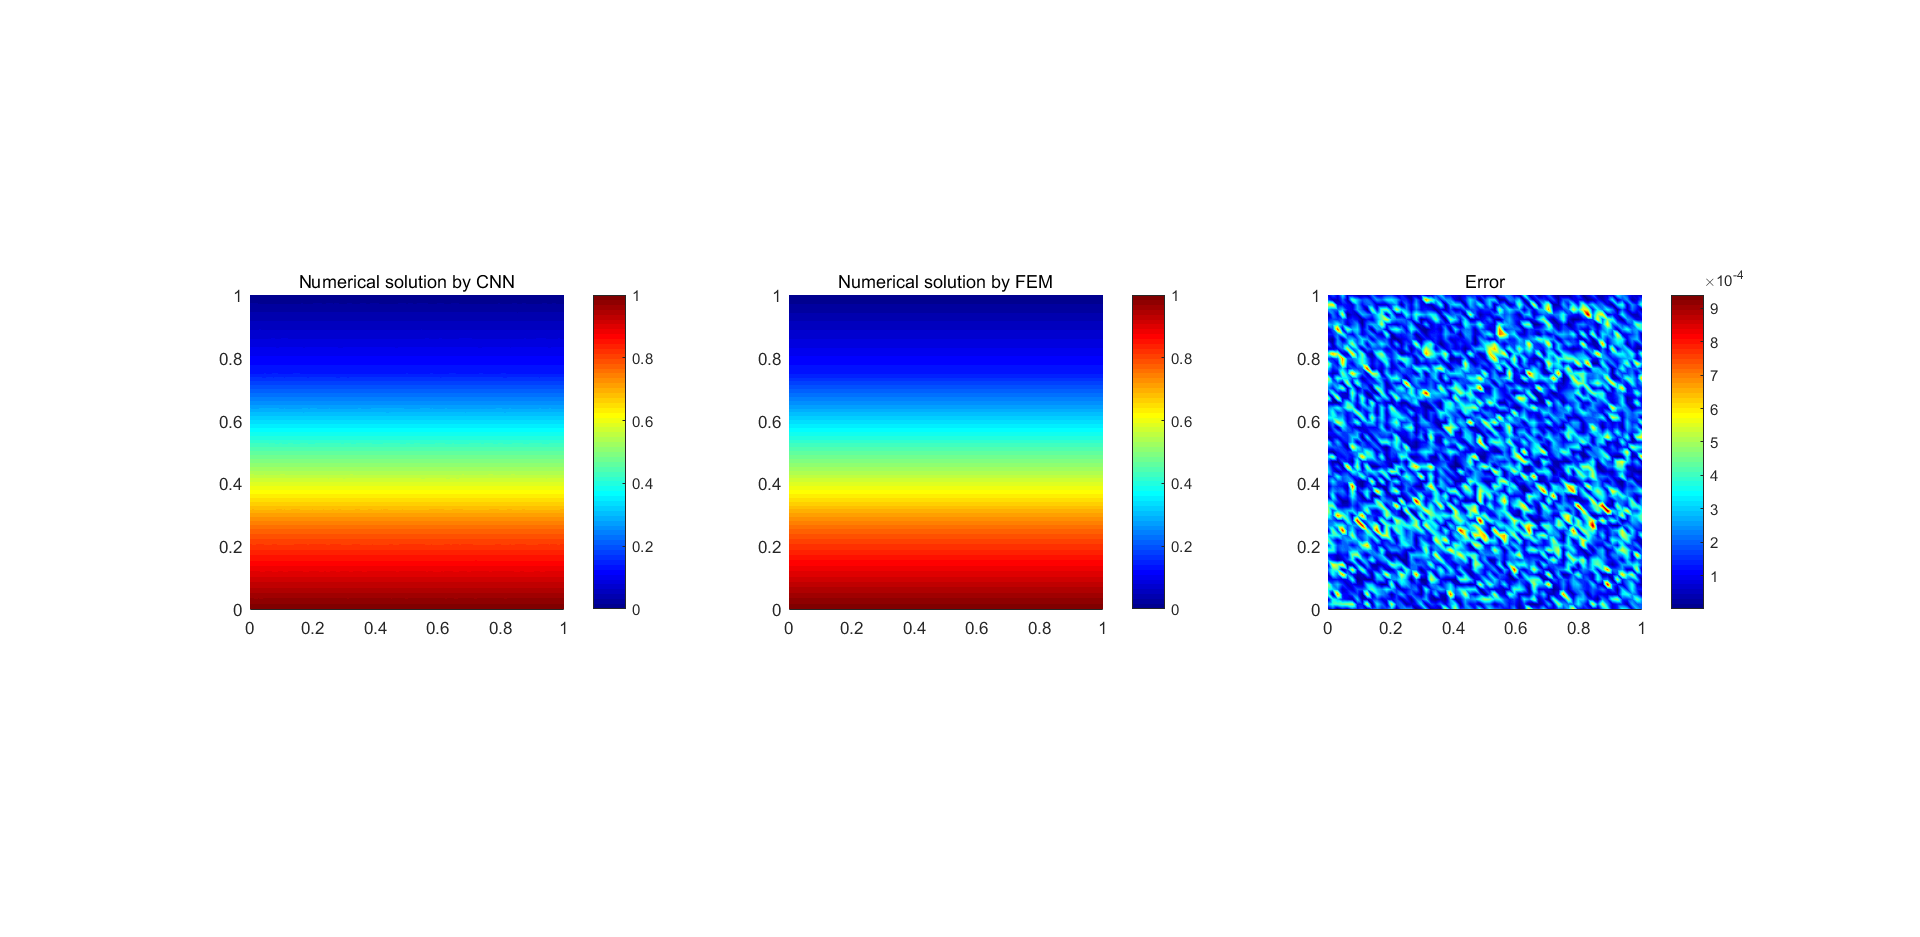
\includegraphics[width=0.65\textwidth]{figures/Darcy_CNN/Darcy_CNN_2000__Adam_nonlinear.png}
	\caption{Comparison of the solutions obtained by CNN with and without activation function by Adam method (Top: without activation, Bottom:  with activation).}
\end{figure}

\begin{figure}[!htbp]
	\centering
	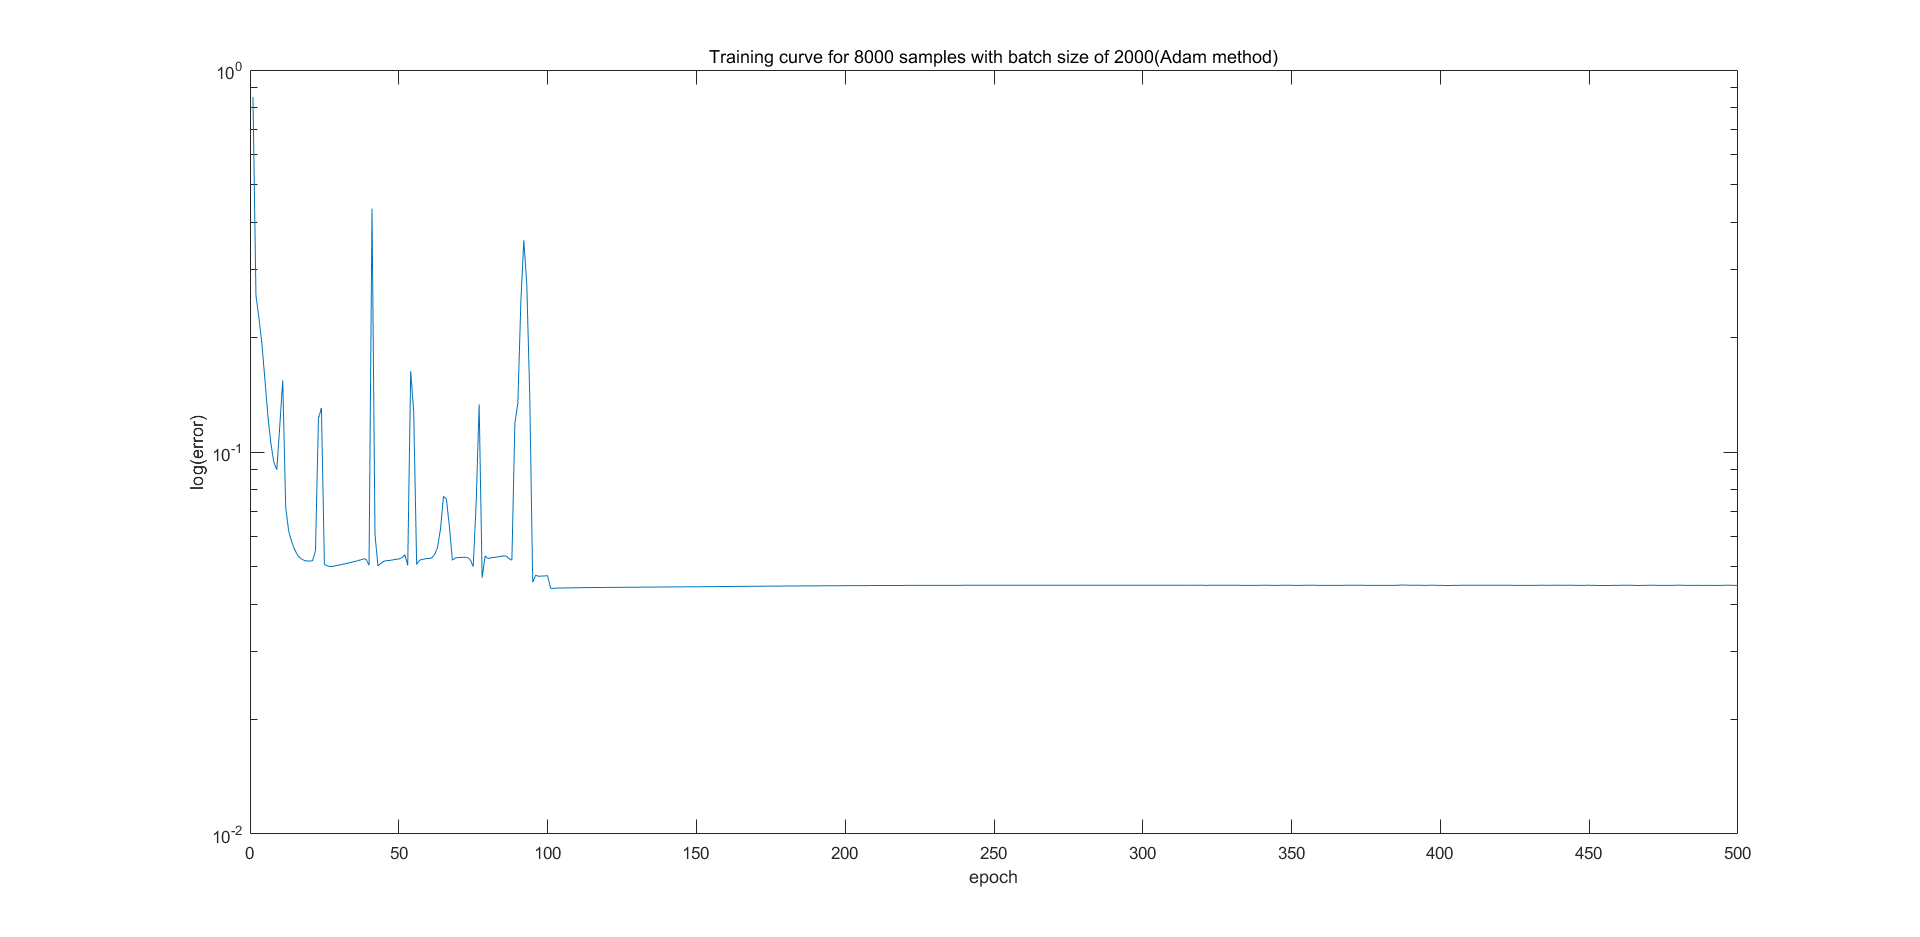
\includegraphics[width=0.45\textwidth]{figures/Darcy_CNN/darcy_loss_2000_adam.png}
	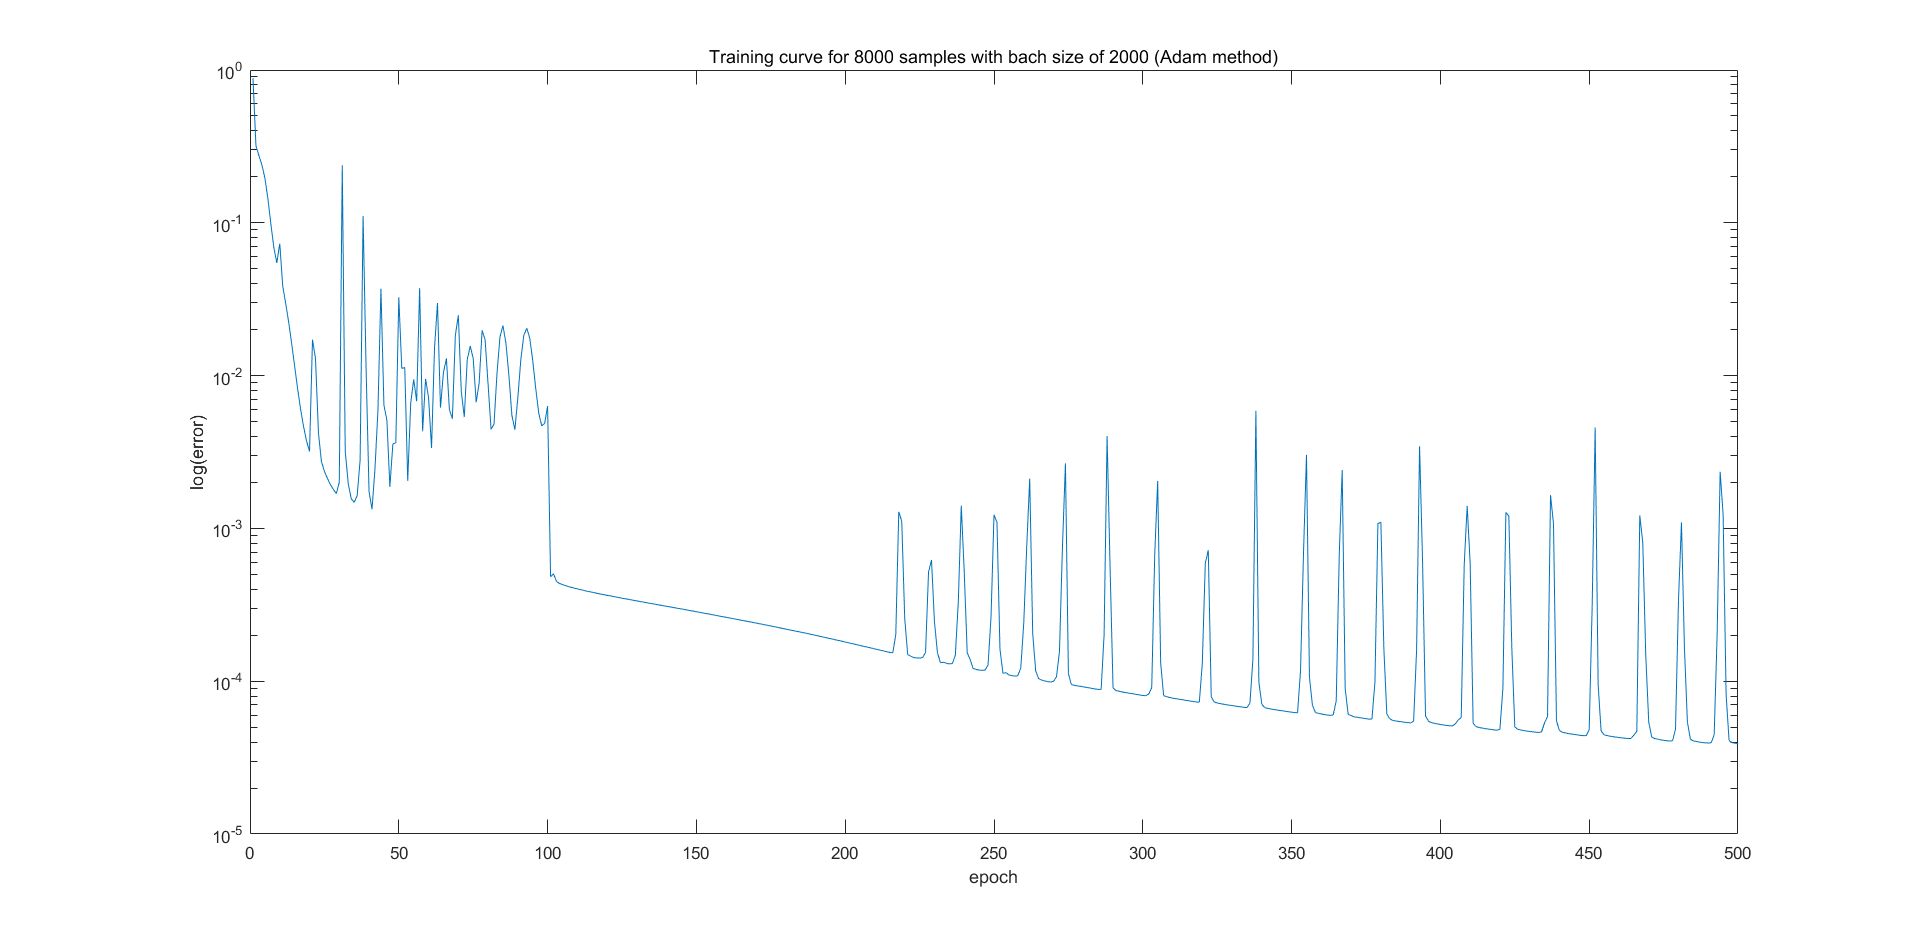
\includegraphics[width=0.45\textwidth]{figures/Darcy_CNN/darcy_loss_2000_adam_nonlinear.png}
	\caption{Training curves  with and without activation function by Adam method (Left: without activation, Right:  with activation).}
\end{figure}

	\begin{figure}[!htbp]
	\centering
	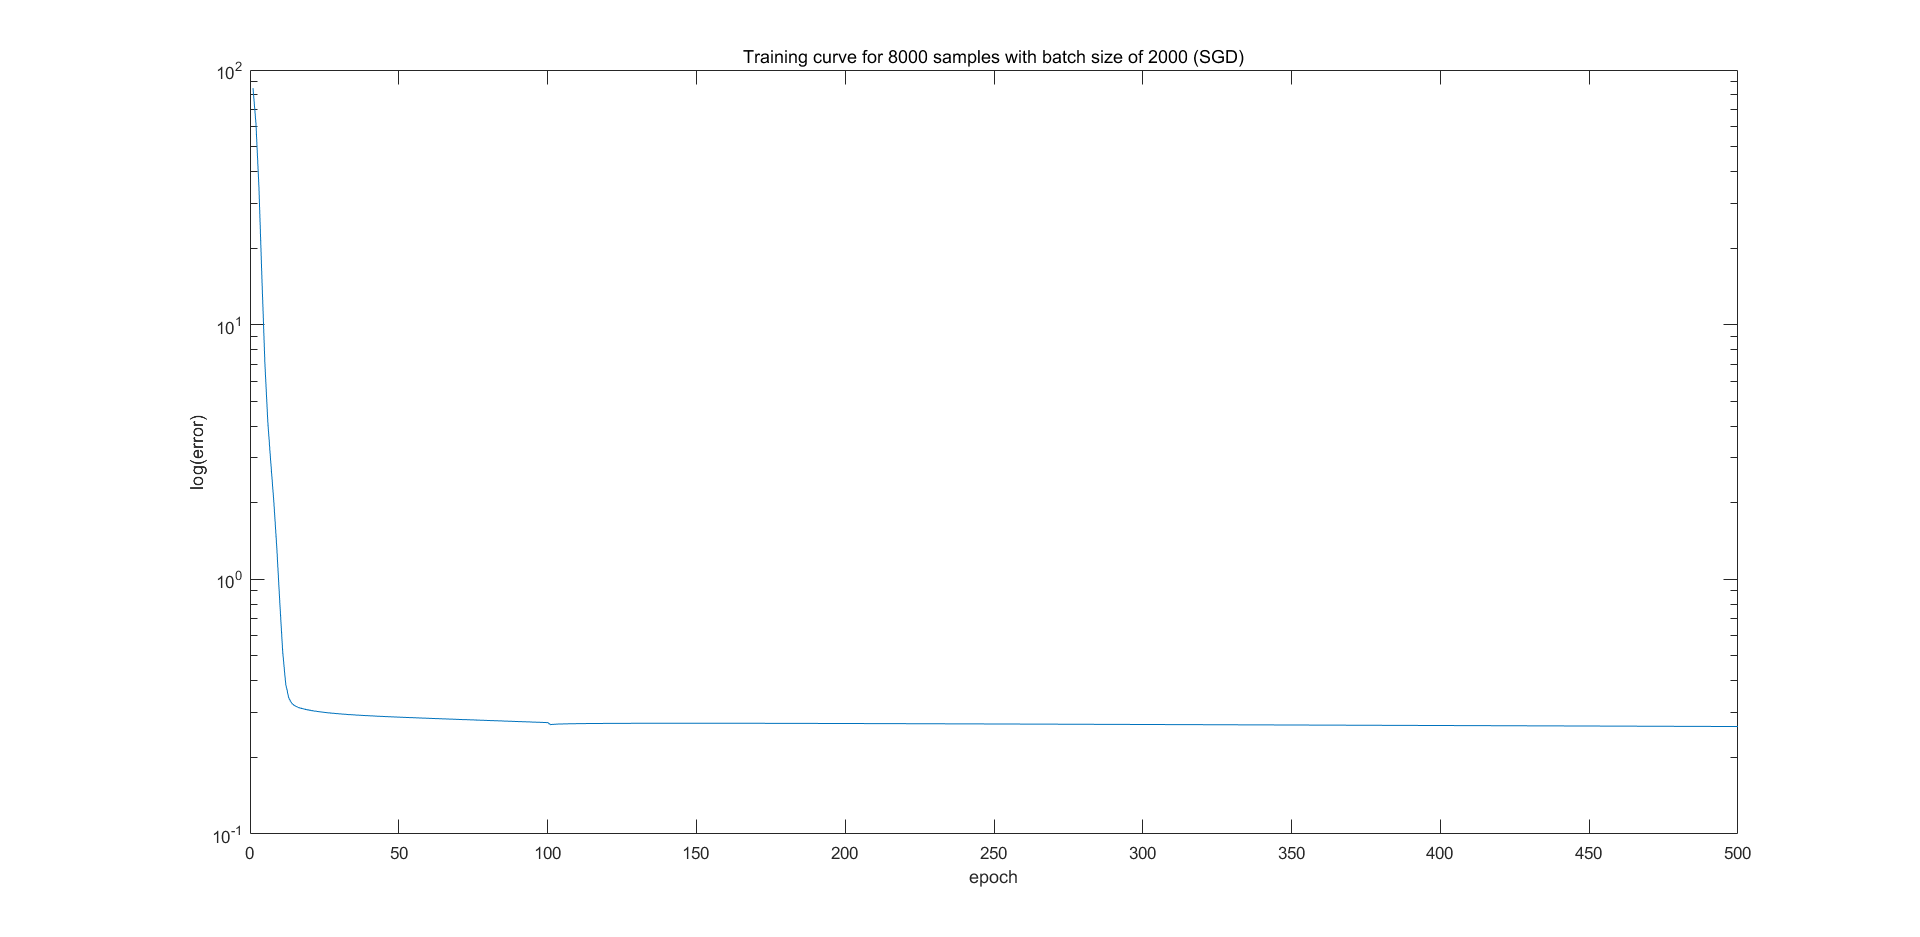
\includegraphics[width=0.45\textwidth]{figures/Darcy_CNN/darcy_loss_2000_SGD.png}
	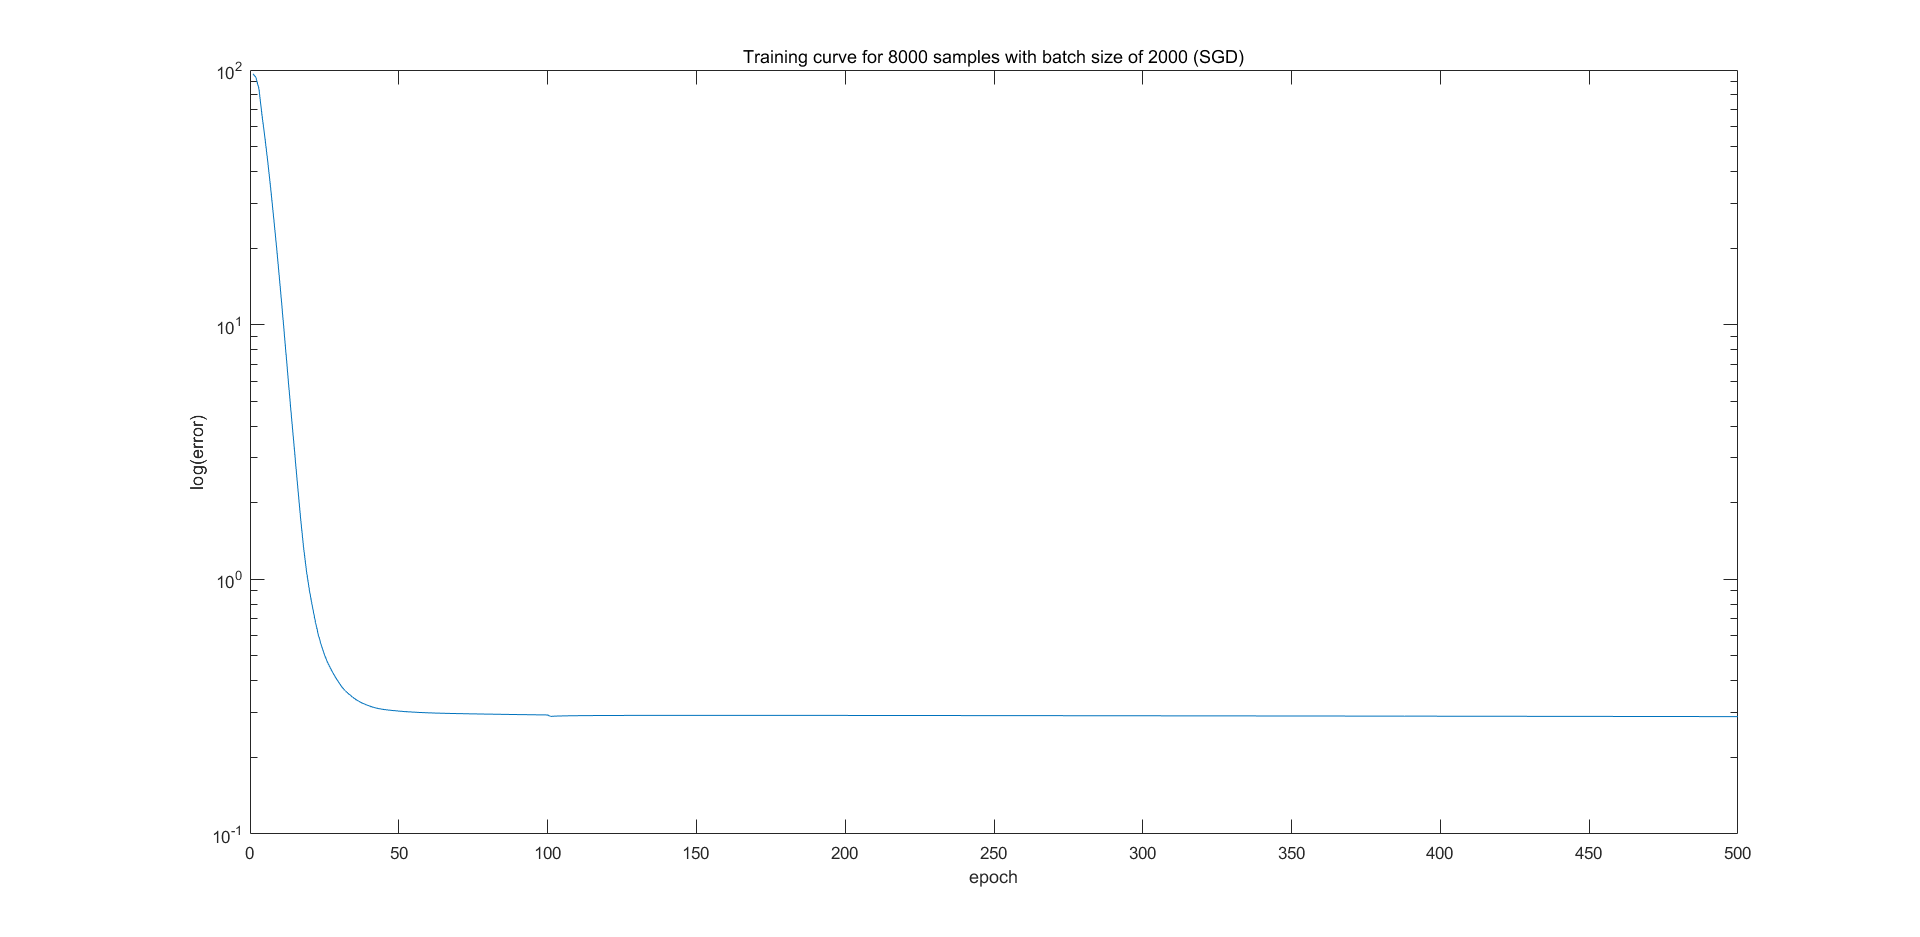
\includegraphics[width=0.45\textwidth]{figures/Darcy_CNN/darcy_loss_2000_SGD_nonlinear.png}
	\caption{Training curves  with and without activation function by SGD method (Left: without activation, Right:  with activation).}
\end{figure}

Below we consider the decoding process as the transpose of the encoding process.
\begin{breakablealgorithm}
	\caption{$u={\rm DarcyCNN_{transpose}}(\kappa; f_d, coarse\_grid\_size,)$}
	\label{alg:mgnet}
	\begin{algorithmic}
		\State Initialization:  $\kappa$
		%		\State Initialization $u^{1,0}$
		%		\For{$ = 1:N_{epoch}$}
		%		\For{$i = 1:\nu_$}
		\State Encode
		\begin{equation}
		u^{} = K^{3}  \ast_2   K^{ 2}\ast  (K^{ 1}\ast \kappa).
		\end{equation}
		
		%		\EndFor
		\State Restriction to the coarse grid
		\begin{equation}
		u^{} =   W u^{}
		\end{equation}
		\State
		Convolution on the coarse grid
		\begin{equation}
		u^{} =   K^{ 5}\ast K^{ 4}\ast u^{}.
		\end{equation}
		\State Decode
		\begin{equation}
		u^{} =  K^{ 1,T} \ast K^{ 2,T}\ast K^{3}  \ast_2^T (W^{ T}  K^{ 4,T}\ast K^{ 5,T}\ast u^{}).
		\end{equation}
		%		\EndFor
	\end{algorithmic}
\end{breakablealgorithm}
Where $K^T$ is the transpose of kernel $K$. For a kernel with size of $3 \times 3$ without padding, its transpose is the central symmetry of itself with 2 paddings.\\

In this network, the parameters are 13 million and 6.5 million respectively.

	\begin{figure}[H]
		\centering
		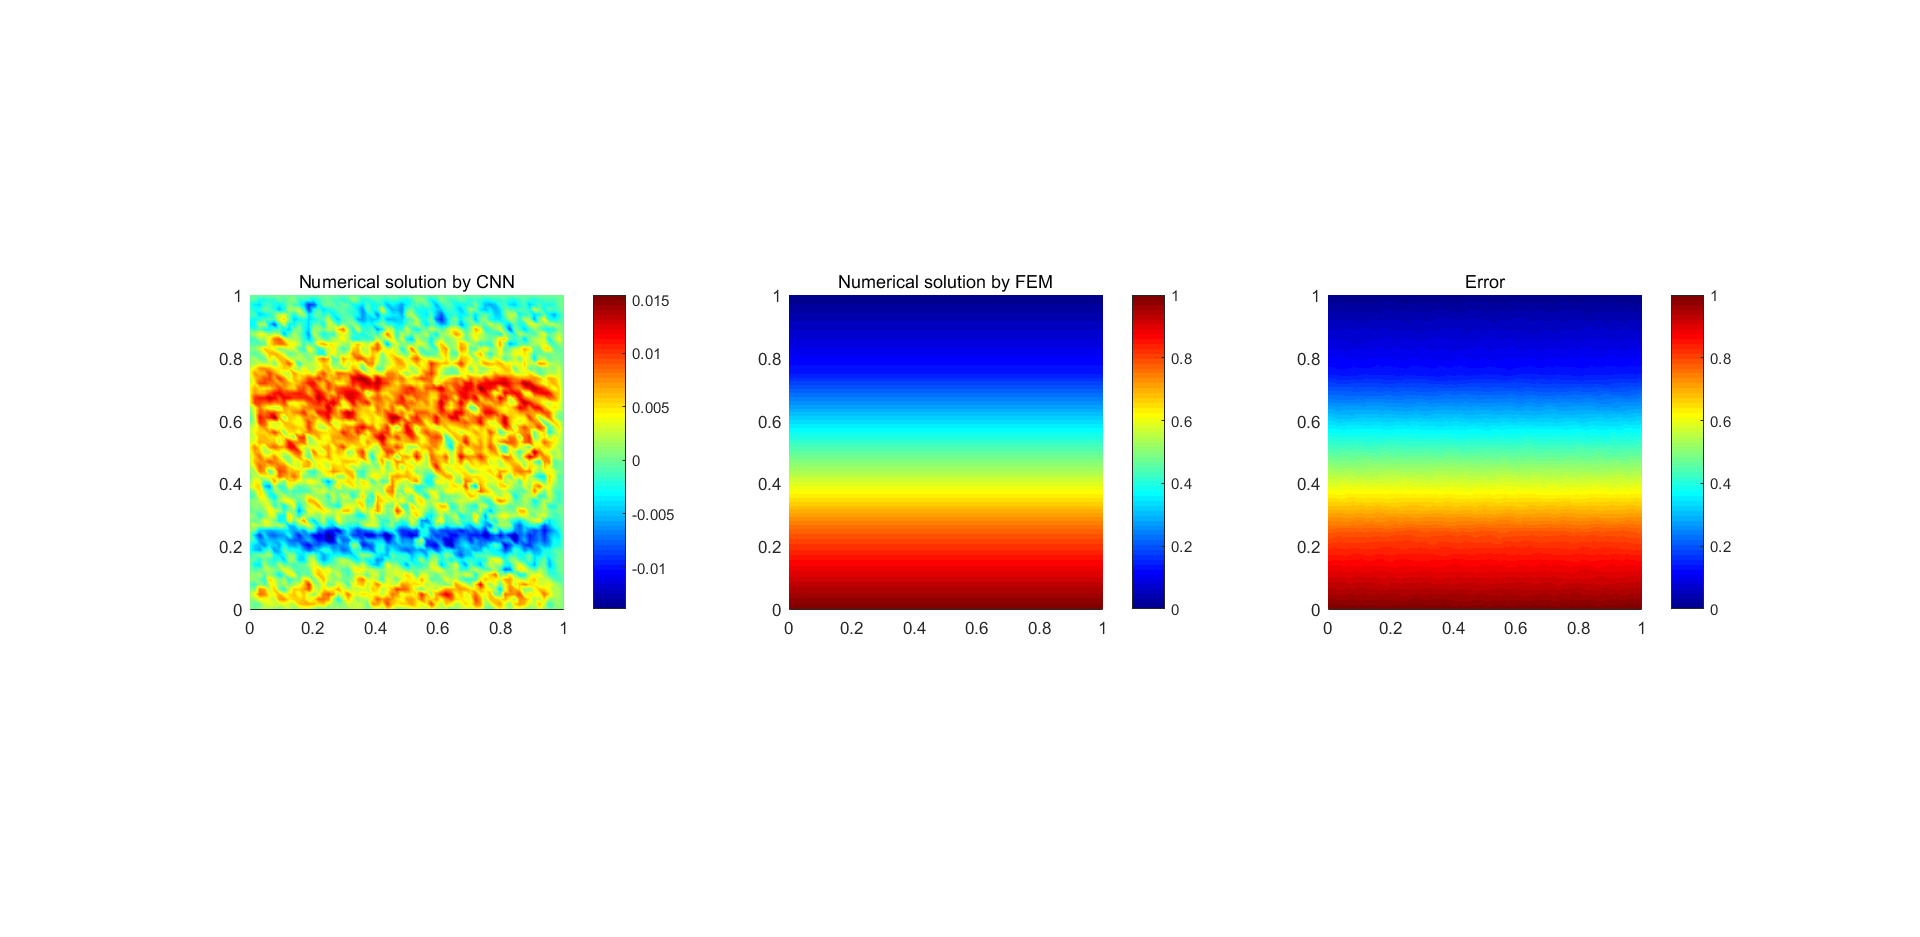
\includegraphics[width=0.45\textwidth]{figures/Darcy_CNN/Darcy_transpose_value_mean.png}
		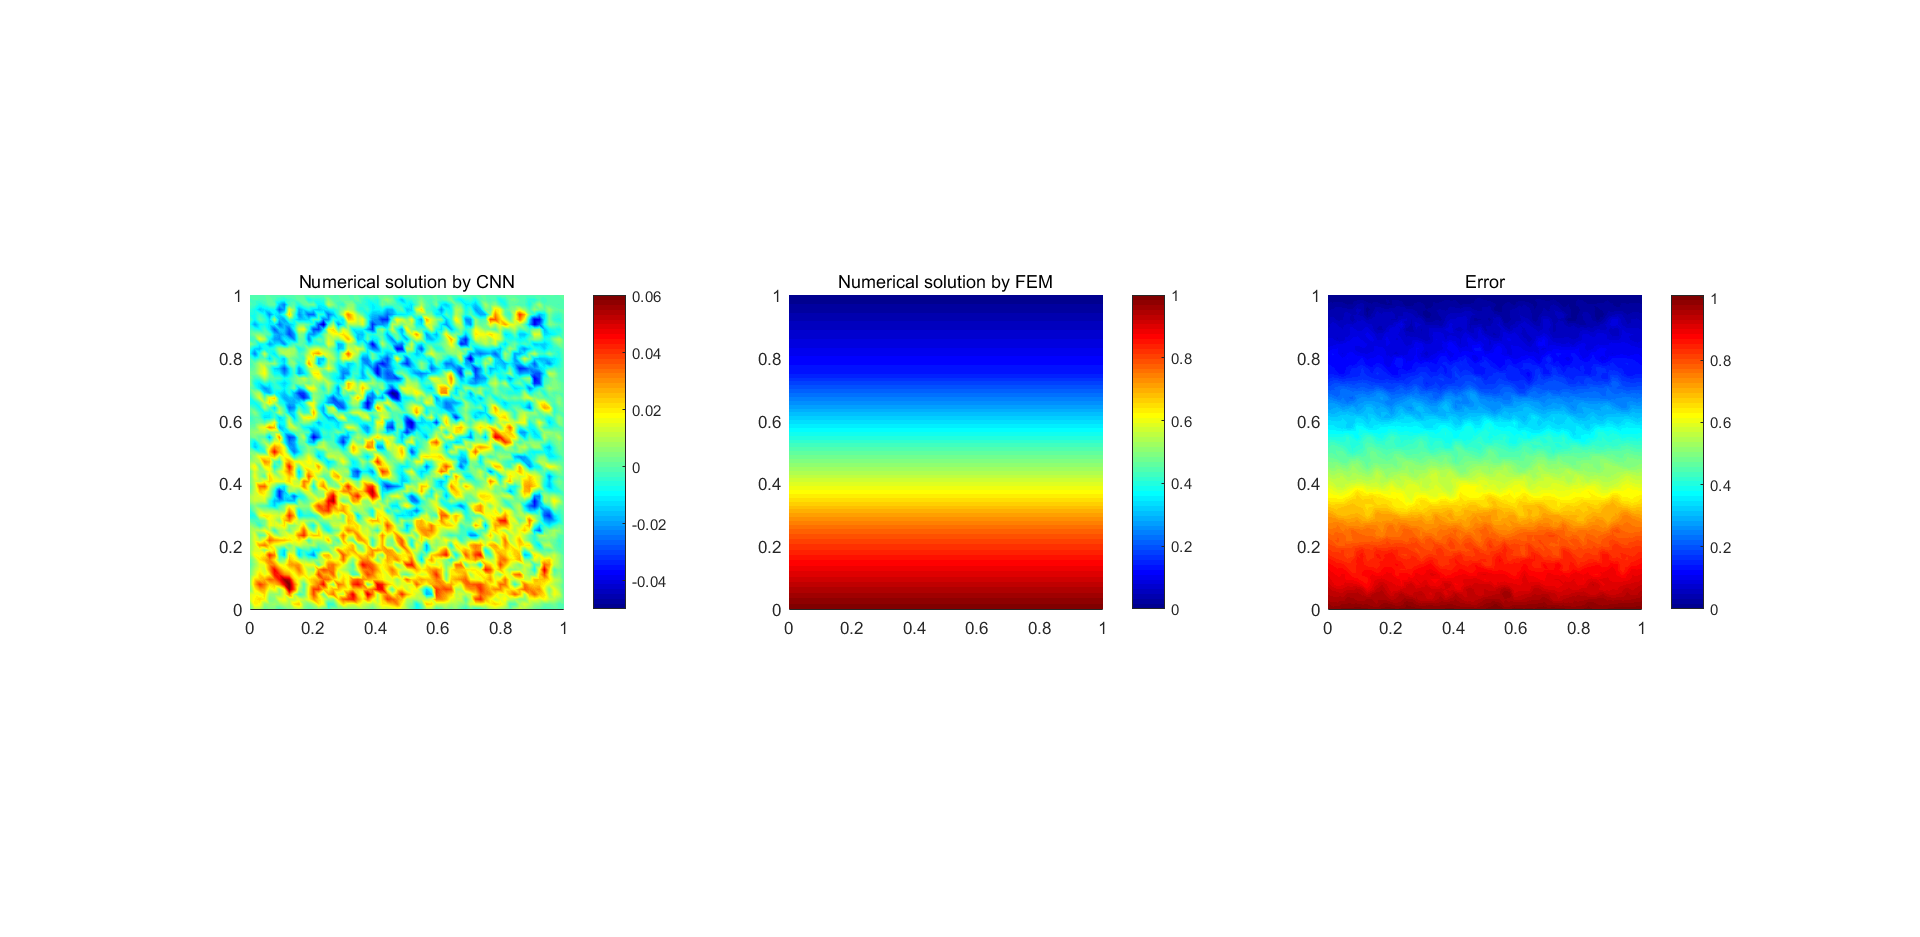
\includegraphics[width=0.45\textwidth]{figures/Darcy_CNN/Darcy_transpose_novalue_mean.png}
		\caption{Comparison of solutions obationed by FEM and neural network including transpose(Left: Transposed parameters untrained, Right: Transposed parameters trained) with zero-mean input.}
	\end{figure}
	
	\begin{figure}[H]
		\centering
		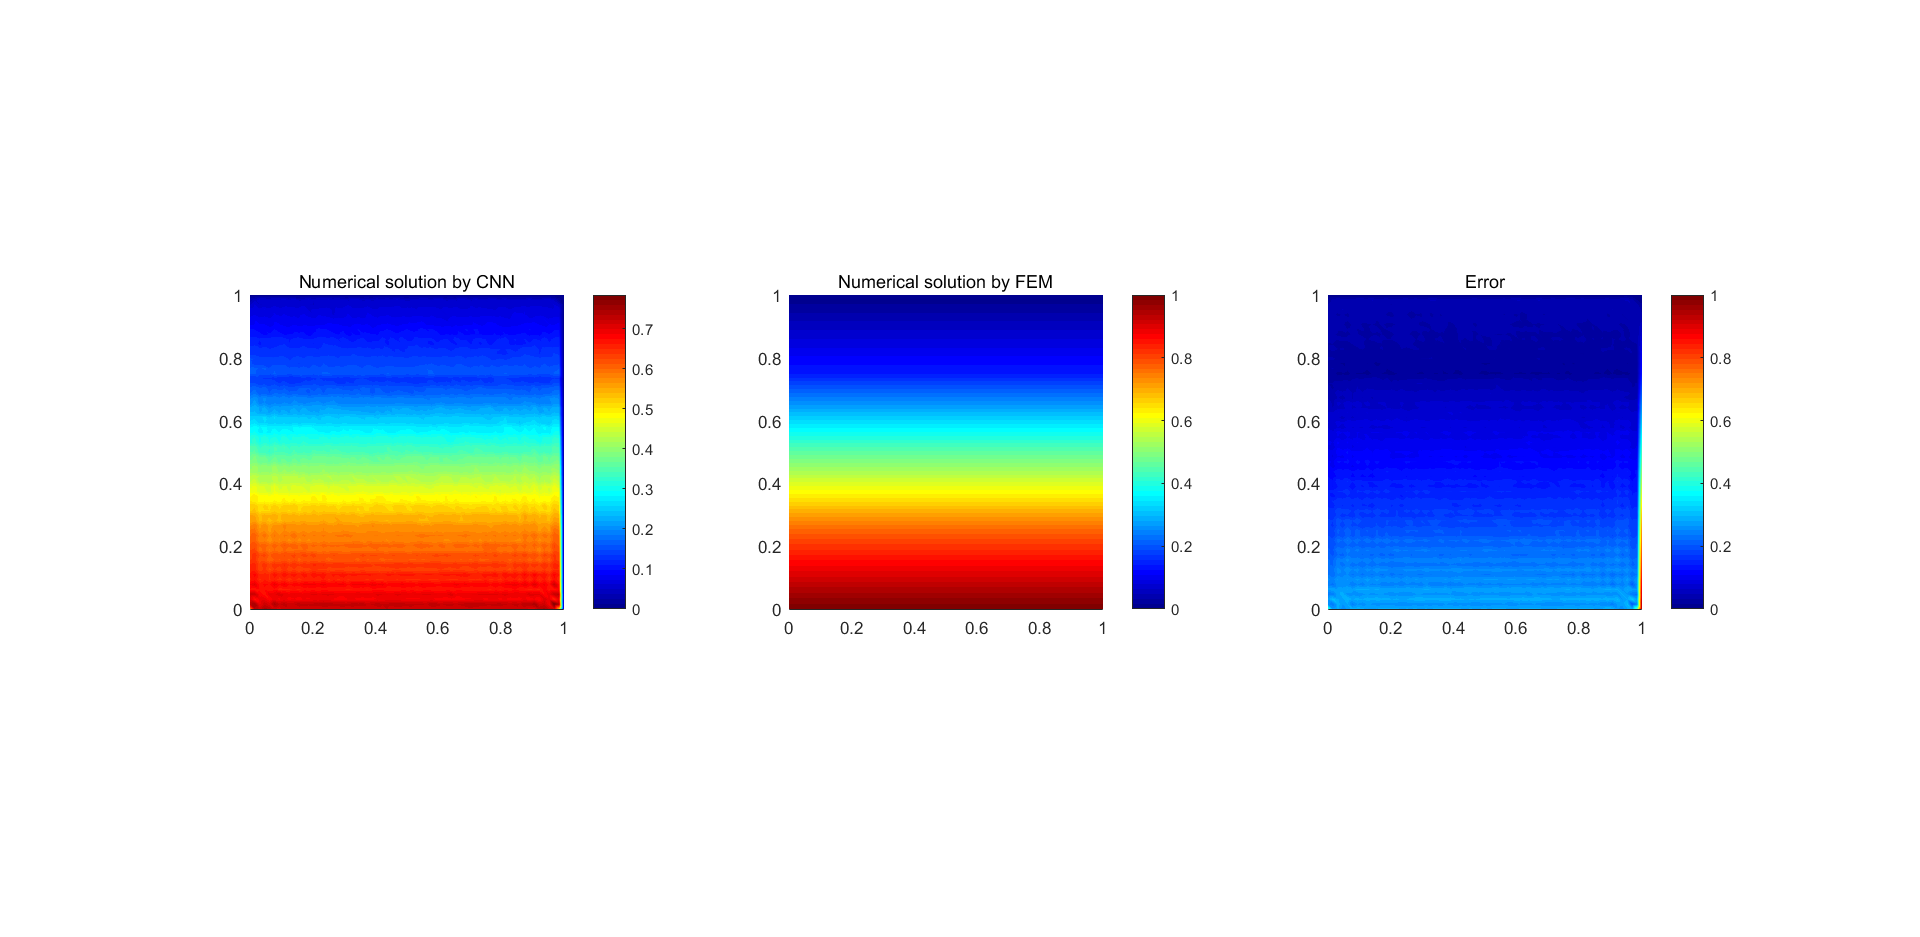
\includegraphics[width=0.45\textwidth]{figures/Darcy_CNN/Darcy_transpose_value.png}
		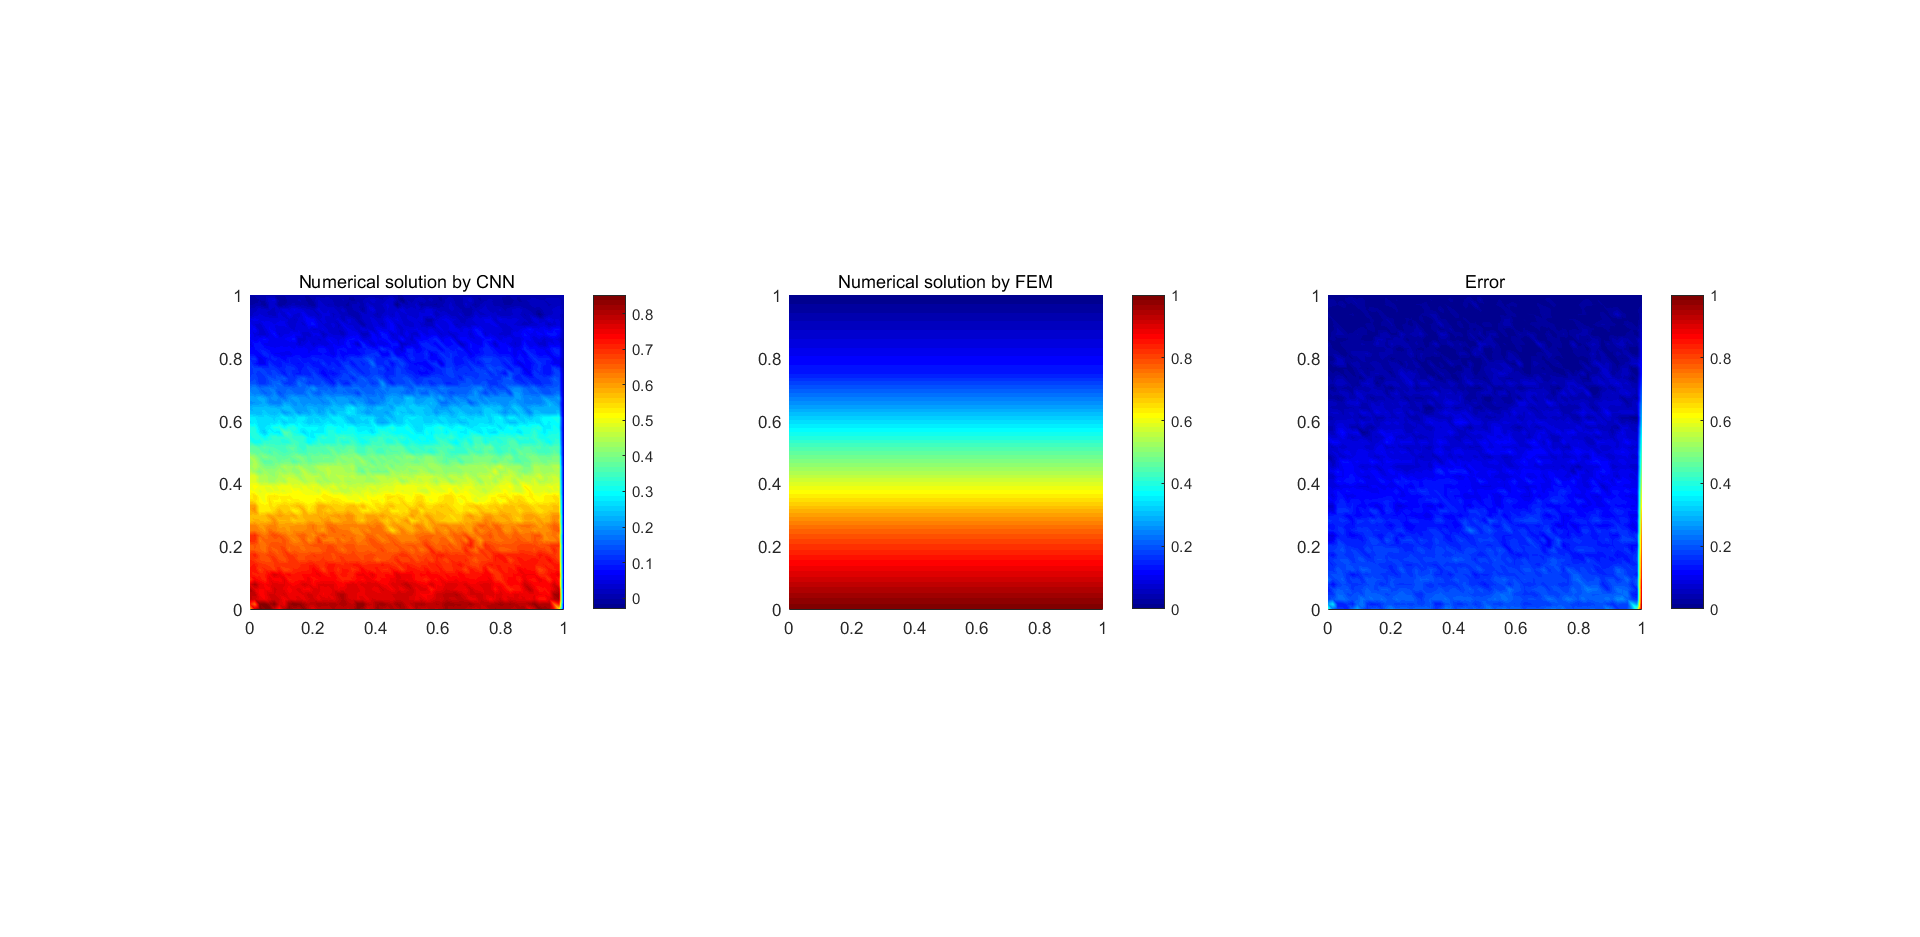
\includegraphics[width=0.45\textwidth]{figures/Darcy_CNN/Darcy_transpose_novalue.png}
		\caption{Comparison of solutions obationed by FEM and neural network including transpose(Left:  Transposed parameters untrained, Right: Transposed parameters trained) with original input.}
	\end{figure}


The problem we feel confused is that unlike the process in PCA method, what we need to do is to solve a darcy equation, where the input data and output data are in two different fields. Therefore, whether it makes sense that using the encode transpose-encode process to solve this problem.

\newpage
\subsection{PCA and POD}
For the differnence between PCA and POD, here we consider following linear problem
$$
A_i x_i = b_i, \quad i = 1,\cdots,N
$$
Consider the solutions $x_i $ are in a hyperplane $y_i = W\tilde{x}_i+\mu$ where $W \in \mathbb{R}^{d\times d'}, d'\ll d $ and $y_i$ is an approximation of $x_i$. To approximate $x_i$ as closely as possible, i.e. minimize loss function
\begin{equation}\label{lossPOD}
L = \sum_{i}^{N}=\| y_i - x_i\|^2 =  \sum_{i}^{N}=\| W\tilde{x}_i +\mu - x_i\|^2
\end{equation}
Then, the best choice of $\tilde{x}_i $ and $\mu$ is
$$
\mu = \frac{1}{N}\sum_{i}^{N}x_i = \bar{x}, \quad
\tilde{x}_i = W^T(x_i-\bar{x})
$$
Then \ref{lossPOD} can rewritten as
$$
L =  \sum_{i}^{N}=\| WW^T(x_i-\bar{x}) +\bar{x} - x_i\|^2 .
$$
The choice of $W$ is the same as PCA method.\\

For the linear problem $Ax=b$, we consider $x = W\tilde{x}+\bar{x}$ and premultiplicate $W^T$ on the eqauation, we get
$$
W^TAW\tilde{x} = W^T(b-A\bar{x}).
$$
Solve the equation above and with the decoder, we can get the approximation of the solution as
$$
x \approx W\tilde{x} + \bar{x}.
$$
In the POD, we consier the solution in the specific hyperplane $y_i = W\tilde{x}_i$, then the low-dimension solution $\tilde{x}$ satisfies
$$
W^TAW\tilde{x} = W^Tb
$$
Apply the decoded to get the approximation solution as
$$
x = W\tilde{x}
$$
For the construction of CNN to solve this problem, the matrix A is associated with $\kappa$ and can be regarded as a linear mapping of $\kappa$, and the right side term $b$ is fixed.

%Here for a input $\kappa$, I wonder the encoded is processed on $\kappa$, or on a linear  mapping of $\kappa$ which approximate the solution $x$. As we all know, the traditional encode-decode process is all about $x$. However, here we need to apply the encoder on $\kappa$ and have some extra computation to solve the equation in a lower dimension. Finally we apply the decoder to get the approximation of the solution.
\subsection{Mgnet-encoder}
In order to make the distance between the approximate solution and true solution  as small as possible, i.e. minimize loss function
$$
L = \sum_{i}^{N} \| g  \circ f(x_i) - x_i \|
$$
If we fix the decoder as a linear function, i.e.
$$
g(y) = Wy + b
$$
Hdre, we use the following MgNet as the encoder
\begin{breakablealgorithm}%[!htb]
	\caption{$\mu^J = {\text{MgNet}}(f; J,\nu_1, \cdots, \nu_J)$}
	\label{alg:L-Slash11d}
	\begin{algorithmic}
		\State Set up
		$$
		f^1 = {\color{red} \theta\ast} f, \quad \mu^{1}=0. 
		$$
		\State Smoothing and restriction from fine to coarse level (nested)
		\For{$\ell = 1:J$}
		\For{$i = 1:\nu_\ell$}
		\State
		\begin{equation}\label{eq:smoothing}
		\mu^{\ell} \leftarrow \mu^{\ell} + S^\ell \ast (f^\ell - A_\ell \ast \mu^{\ell}).
		\end{equation}
		\EndFor
		\State Form restricted residual and set initial guess:
		$$
		\mu^{\ell+1} \leftarrow \Pi_{\ell}^{\ell+1}\mu^\ell , \quad
		f^{\ell+1} \leftarrow R^\ell \ast_2 (f^\ell -  A_\ell \ast
		\mu^{\ell}) + A_{\ell+1}\ast 	\mu^{\ell+1} ,    %A_{\ell+1} = R       \ast_2 A_\ell \ast (R\ast_2^\top).
		$$
		\EndFor
		\State
		Finally, we ultilize the Adaptive average pooling to let the number of element in every channel of $\nu^J$ be 1.
		$$\nu^J = Avg \ast \nu^J$$
	\end{algorithmic}
\end{breakablealgorithm}
Here, $\mu_J$ is the reduced vector. For the decoder, we denote $(u^l,f^l)$ as a new variable.
Then we can induce that
$$\mu^{l+1}=\phi^{l+1}\mu^l + \xi^{l+1}f^{l+1}$$
$$f^{l+1} = R^l f^l + M^l \mu^l $$
where $\phi^{l+1}= (N^{l+1})^{v_{l+1}}\Pi_l^{l+1}, N^{l+1}= I - S^{l+1}A^{l+1} $, $\xi^{l+1}=\big(\sum_{i=1}^{v_{l+1}-1}(N^{l+1})^i\big)S^{l+1}$ and $M^l = A^{l+1}\Pi_l^{l+1} - R^lA^l$.

We can also rewritten the equation above as
\[
\left( \begin{array}{l}
f^{l+1} \\
\mu^{l+1}
\end{array} \right) = \left( {\begin{array}{*{20}{c}}
	R^l & M^l\\
	\xi^{l+1}R^l&\phi^{l+1}+\xi^{l+1}M^l
	\end{array}} \right)\left( \begin{array}{l}
f^{l}\\
\mu^{l}
\end{array} \right), \quad
\left( \begin{array}{l}
f^{1} \\
\mu^{1}
\end{array} \right) = \left( {\begin{array}{{c}}
	\theta \\
	\xi^{1}\theta
	\end{array}} \right)\left( \begin{array}{l}
f\\
\end{array} \right)
\]
We can then define the mgnet-decoder as
\begin{breakablealgorithm}%[!htb]
	\caption{$f = {{\rm MgNet_{transpose}}}(u^J; J,\nu_1, \cdots, \nu_J)$}
	\begin{algorithmic}
		\State Transpose of Adapative Average pooling
		$$\mu^J = Avg^T \ast \nu^J $$
		\State Prolongation back to the fine level 
		\State 
		$$
		f^{J-1} = R^{J-1, T}\xi^{J, T}\mu^J,  \qquad \mu^{J-1} = (M^{J-1,T}\xi^{J, T} + \phi^{J-1, T})\mu^{J}
		$$
		\For{$\ell = J-2:1$}
		\State
		\begin{equation}
		\mu^{\ell}= M^{\ell,T}f^{\ell+1} + (M^{\ell,T}\xi^{\ell+1, T} + \phi^{\ell, T})\mu^{\ell+1}.
		\end{equation}
		\State
		\begin{equation}
		f^{\ell} = R^{\ell, T}f^{\ell+1} + R^{\ell, T}\xi^{\ell+1, T}\mu^{\ell+1}
		\end{equation}
		\EndFor
		\State Transpose of pre-convolution:
		$$
		f = \theta^T \ast f^1 + \theta^T \ast \xi^{1,T} \mu^1
		$$
	\end{algorithmic}
\end{breakablealgorithm}

\subsection{Numerical results}
Then we have the some results for the following test.

\begin{itemize}
	\item Model equations
	\begin{align*}
	- \nabla \cdot (\kappa \nabla p) & = 0  \qquad \text{in}~~ \Omega \\
	\kappa \nabla p \cdot n &= 0 \qquad \text{on} ~~ \Gamma_\text{N} \\
	p  &= 0 \qquad \text{on} ~~\Gamma_{\text{D}1} \\
	p  &= 1 \qquad \text{on}~~ \Gamma_{\text{D}2} \\
	\end{align*}
	\begin{center}
		\vskip -20pt
		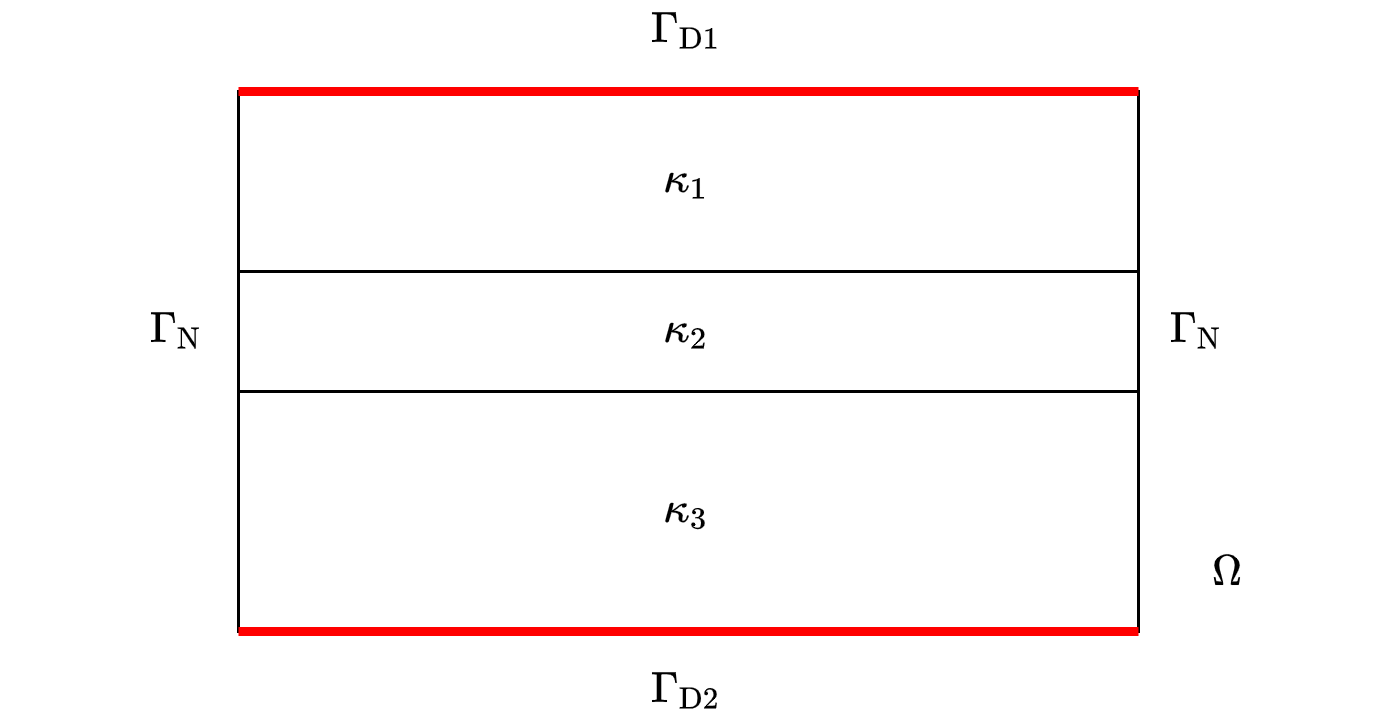
\includegraphics[height=5cm]{figures/Darcy_CNN/Darcy_domain.png}
	\end{center}
\end{itemize}
The loss fucntion is
$$
L = \sum_{i}^{N} \| g  \circ f(x_i) - x_i \|
$$
where $x_i$ is the FEM solution given the permeability $\kappa_i$, $f$ is the Mgnet encoder and $g$ is the Mgnet-Transpose decoder.

\begin{itemize}
	\item Uniformly generate 2000 training samples: $\kappa_1 \sim \mathcal{U}(2.5,7,5), \kappa_2 \sim \mathcal{U}(1,3)$ and $\kappa_3 \sim \mathcal{U}(0.5,1.5)$
	\item Grid size: $33*33 ~ (d=1089)$
	\item Number of training samples: 2000
	\item Number of epochs: 2000
	\item Number of test samples: 500
	\item Mgnet learning rate: $10^{-3}$
	\item DNN learning rate: 0.1
\end{itemize}
Here, we give the results of DNN and MgNet:

\subsubsection{Case 1: Fix J, change $\nu_i$}
Let $J=4,$, number of $\mu$'s channel equals to 10, number of $f$'s channel equals to 1, we test the cases when $\nu_i=1,2,3,4$.
\begin{table}
	\begin{center}
		\begin{tabular}{|c|c|c|c|c|}
			\hline
			& $\nu_i$=1 & $\nu_i$=2 & $\nu_i$=3& $\nu_i$=4 \\
			\hline
			Train loss & 1.1861 $\times 10^{-2}$ & 1.197 $\times 10^{-2}$& 1.0793 $\times 10^{-2}$ & 1.0795 $\times 10^{-2}$\\
			\hline
			Mean rel. errors & 6.358 $\times 10^{-3}$ &6.199 $\times 10^{-3}$ &5.947 $\times 10^{-3}$ &6.010 $\times 10^{-3}$ \\
			\hline
		\end{tabular}\caption{Training errors and test errors(3456 parameters).}
	\end{center}
\end{table}

\subsubsection{Case 2: Fix $\nu_i$, change J}
Let $\nu_i$=2, number of $\mu$'s channel equals to 10, number of $f$'s channel equals to 1, we test the cases when $J=3,4,5,6$
.\begin{table}
	\begin{center}
		\begin{tabular}{|c|c|c|c|c|}
			\hline
			& $J=3$ & $J=4$ & $J=5$& $J=6$ \\
			\hline
			Train loss & 1.3235 $\times 10^{-2}$ & 1.1197 $\times 10^{-2}$& 1.0760 $\times 10^{-2}$ & 1.0663 $\times 10^{-2}$\\
			\hline
			Mean rel. errors & 6.613 $\times 10^{-3}$ &6.199 $\times 10^{-3}$ &6.022 $\times 10^{-3}$ &5.956 $\times 10^{-3}$ \\
			\hline
			Number of Para & 2367& 3456& 4545 & 5634\\
			\hline
		\end{tabular}\caption{Training errors and test errors for various J.}
	\end{center}
\end{table}
\begin{figure}[H]
	\centering
	\includegraphics[width=0.6\textwidth]{figures/Darcy_CNN/loss_J.png}
	\caption{Training curves for various J=3,4,5,6.}
\end{figure}
\subsubsection{Case 3: Change number of $u$'s channel}
Let $\nu_i$=2, number of $f$'s channel equals to 1, $J=4$, we test the cases when the number of $\mu$'s channel equals to $10,20,30,40$
.\begin{table}
	\begin{center}
		\begin{tabular}{|c|c|c|c|c|}
			\hline
			& $n_u=10$ & $n_u=20$ & $n_u=30$& $n_u=40$ \\
			\hline
			Train loss & 1.1197 $\times 10^{-2}$ & 1.0772 $\times 10^{-2}$& 0.9634 $\times 10^{-2}$ & 0.8550 $\times 10^{-2}$\\
			\hline
			Mean rel. errors & 6.199$\times 10^{-3}$ & 6.091 $\times 10^{-3}$ &5.796 $\times 10^{-3}$ &5.574$\times 10^{-3}$ \\
			\hline
			Number of Para & 3456& 12276& 26496 & 71136\\
			\hline
		\end{tabular}\caption{Training errors and test errors for various number of $u$'s channel.}
	\end{center}
\end{table}

\begin{figure}[H]
	\centering
	\includegraphics[width=0.6\textwidth]{figures/Darcy_CNN/loss_u_channel.png}
	\caption{Training curves for various number of $u$'s channel.}
\end{figure}

\subsubsection{Case 4: DNN results}
For the one-layer DNN, we test the cases when the number of reduced dimension is $10, 20, 30 ,40$.
.\begin{table}[H]
	\begin{center}
		\begin{tabular}{|c|c|c|c|c|}
			\hline
			& 10 & 20 & 30& 40 \\
			\hline
			Train loss & 1.0584 $\times 10^{-2}$ & 0.8902 $\times 10^{-2}$& 0.7296$\times 10^{-2}$ & 0.6819 $\times 10^{-2}$\\
			\hline
			Mean rel. errors & 6.110$\times 10^{-3}$ & 5.852 $\times 10^{-3}$ &5.571$\times 10^{-3}$ &5.470$\times 10^{-3}$ \\
			\hline
			Number of Para & 10890& 21780& 32670 & 54450\\
			\hline
		\end{tabular}\caption{Training errors and test errors for various reduced dimension.}
	\end{center}
\end{table}
\textbf{In this test, we noticed that the weight obtained by DNN almost satisfies the orthogonality, and the weight obtained by MgNet also has the trendency to satisfy the orthogonality where the elements on the diagnol close to 1 and the non-diagol elements close to 0.}

\subsubsection{Case 5: POD results}
For the POD method, we test the cases when the number of reduced basis is $10, 20, 30 ,40$
.\begin{table}
	\begin{center}
		\begin{tabular}{|c|c|c|c|c|}
			\hline
			& 10 & 20 & 30& 40 \\
			\hline
			Mean rel. errors & 6.345$\times 10^{-3}$ & 6.111 $\times 10^{-3}$ &5.918$\times 10^{-3}$ &5.788$\times 10^{-3}$ \\
			\hline
		\end{tabular}\caption{Test results for various reduced basis number.}
	\end{center}
\end{table}

However, there exists a problem for this numerical test because the variance of every entry  of the solution is actually verly small ($10^-5$). From the results above, we can only infer that CNN can use less paramters to obtain the weight than DNN does. To illustrate this conclusion, we consider further numerical tests.

\subsection{Extend tests}
Here we let the source term of the equation be 1, i.e., 
\begin{itemize}
	\item Model equations
	\begin{align*}
		- \nabla \cdot (\kappa \nabla p) & = 1  \qquad \text{in}~~ \Omega \\
		\kappa \nabla p \cdot n &= 0 \qquad \text{on} ~~ \Gamma_\text{N} \\
		p  &= 0 \qquad \text{on} ~~\Gamma_{\text{D}1} \\
		p  &= 1 \qquad \text{on}~~ \Gamma_{\text{D}2} \\
	\end{align*}
	\begin{center}
		\vskip -20pt
		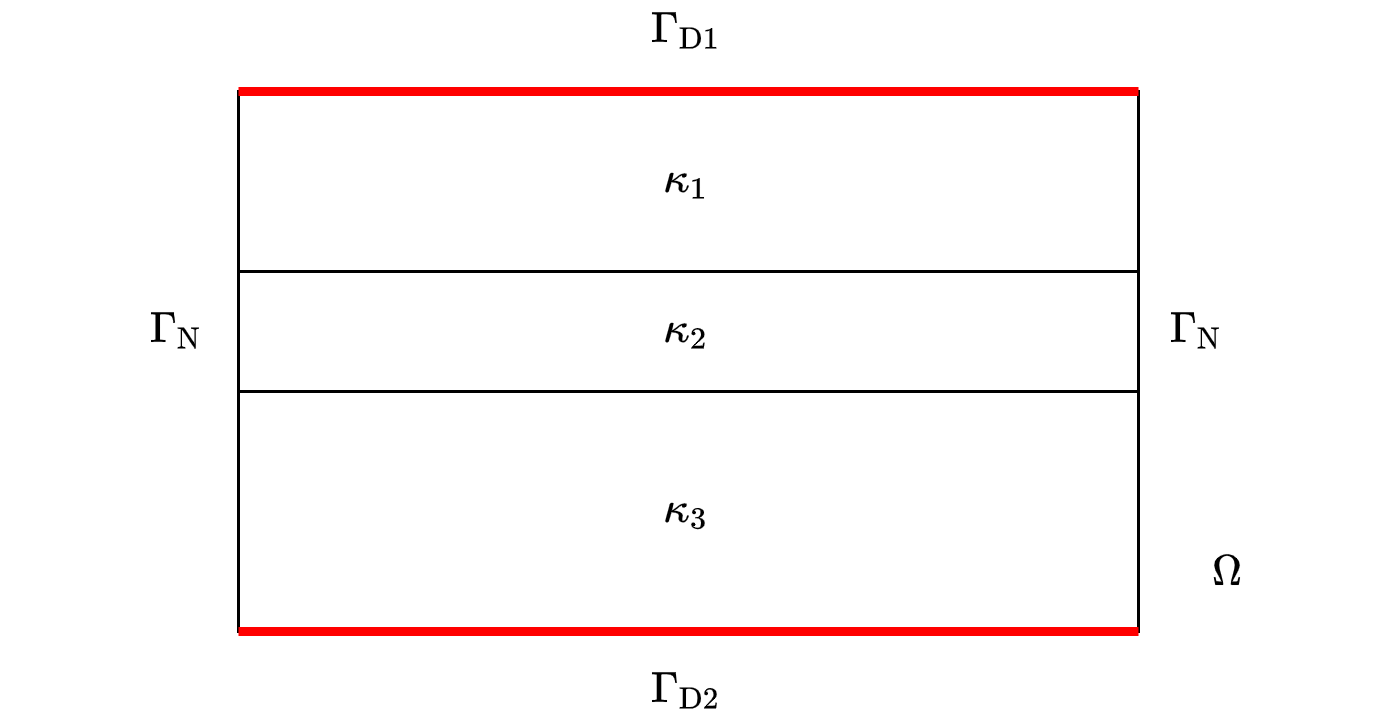
\includegraphics[height=5cm]{figures/Darcy_CNN/Darcy_domain.png}
	\end{center}
\end{itemize}

Then the variance of every entry is about 0.11, which is lager than the previous case. Fix the number of $u$'s channel as 1, we have the following results.

\subsubsection{Case 1: Change $\nu_i$}
\begin{table}[H]
	\begin{center}
		\begin{tabular}{|c|c|c|c|c|}
			\hline
			$\nu_i$& 1& 2 & 3& 4 \\
			\hline
			Train loss & 53.4168 & 55.3550 & 53.3935 & 53.8467\\
			\hline
			%			Mean rel. errors & 6.110$\times 10^{-3}$ & 5.852 $\times 10^{-3}$ &5.571$\times 10^{-3}$ &5.470$\times 10^{-3}$ \\
			%			\hline
			Number of Para & 135 & 135 & 135 & 135\\
			\hline
		\end{tabular}\caption{Training errors for various reduced dimension(lr = $10^{-2}$).}
	\end{center}
\end{table}
\subsubsection{Case 2: Change $J$}
\begin{table}[H]
	\begin{center}
		\begin{tabular}{|c|c|c|c|c|}
			\hline
			J& 3& 4 & 5& 6 \\
			\hline
			Train loss & 44.7566 & 55.3550 & 66.2886& 78.9738\\
			\hline
			%			Mean rel. errors & 6.110$\times 10^{-3}$ & 5.852 $\times 10^{-3}$ &5.571$\times 10^{-3}$ &5.470$\times 10^{-3}$ \\
			%			\hline
			Number of Para & 99 & 135 & 171 & 207\\
			\hline
		\end{tabular}\caption{Training errors for various reduced dimension(lr = $10^{-2}$).}
	\end{center}
\end{table}
\subsubsection{Case 3: DNN results}
.\begin{table}[H]
	\begin{center}
		\begin{tabular}{|c|c|c|c|c|}
			\hline
			& 10 & 20 & 30& 40 \\
			\hline
			Train loss & 60.4035  & 50.5609 & 45.3879 & 42.3671 \\
			\hline
%			Mean rel. errors & 6.110$\times 10^{-3}$ & 5.852 $\times 10^{-3}$ &5.571$\times 10^{-3}$ &5.470$\times 10^{-3}$ \\
%			\hline
			Number of Para & 10890& 21780& 32670 & 54450\\
			\hline
		\end{tabular}\caption{Training errors for various reduced dimension(lr = $10^{-5}$).}
	\end{center}
\end{table}
\subsection{Some disscusion about the orthogonality}
Review that the loss function is 
$$
L = \Sigma_{i=1}^N \| WW^Tx_i  -x_i \| ^2
$$
where $W\in \mathbb{R}^{d\times k}, k \ll d$. Here the matrix $A=WW^T$ is a symmetric positive semi-definite matrix, which have the following decomposition
$$
Q^TAQ  = \Lambda
$$
where Q is a orthogonal matrix and $\Lambda = diag(x_k, 0)$ is a diagnoal matrix, $x_k$ ia a strictly positive  $k$ element vector.

Then the loss function can be written as
$$
\begin{aligned}
L&= \sum x_i^TA^TAx_i - 2x_i^TAx_i +x_i^Tx_i^T\\
&= \sum x_i^TQ \Lambda^2 Q^Tx_i - 2x_i^TQ\Lambda Q^Tx_i
\end{aligned}
$$
To minimize the loss function, for each element of $x_k=(\lambda_i)$, we need to minimize the following problem for each $\lambda_i, i = 1,\cdots, k$
$$
M \lambda_i^2 - 2M \lambda_i
$$
where $M=M(Q,x_i)$ is  positive and depends on $x_i$ and Q. Therefore, $\lambda_i$ should be 1 for the purpose.

Then the original problem is equivalent to maximize the following problem
$$
\begin{aligned}
L & = \sum_{i=1}^{N}x_i^TQ \Lambda Q^T x_i\\
& = \sum_{i=1}^N \sum_{j=1}^k x_i q_j q_j^T x_i\\
& = \sum_{j=1}^k q_j^TXX^T q_j
\end{aligned}
$$
where $X = (x_1,\cdots,x_N)$, $\{q_j\}, j=1,\cdots k$ is the first $k$ columns of orthogonal matrix $Q$.

Then the problem is equivalent to the PCA method which requires the orthogonality, i.e., the orthogonality is a necessary condition to unique the minimizer.

On the other hand, if we consider $A = WW^T$. From above we know that the eigenvalues of $A$ is 1 and 0, and $A$ has a decomposition as $A = WW^T$ where $W$ is not unique.

Without the constaint of orthogonality, this weight $W$ is not unique. Therefore, CNN can generate one of the weight matrix $W_{CNN}$, if this weight matrix is orthogonal, then CNN has no difference from POD method. If not, CNN may be better than POD method.

\subsection{Othogonality is necessary and sufficient}
In the following part, I will prove that the weight matrix must satisfy the orthogonality.

Firstly, for the matrix $A = WW^T$ where $A\in \mathbb{R}^{n\times n}, W \in \mathbb{R}^{n\times r}, r\ll n$. There exists an orthogonal matrix $Q$ and a diagnoal matrix $\Lambda$ such that
$$
A = Q^T \Lambda Q
$$
Then we have $\Lambda = QWW^TQ^T$. Consider the decomposition of $\Lambda$, since the eigenvalues of $A$ is 1 and 0, $\Lambda$ can be written as $diag(e_r, 0)$ where $e_r$ is a r-dim vector of all ones. We have
$$
\Lambda= \left( \begin{array}{c}
	A_r \\
	A_{n-r}
	\end{array}\right) (A_r^T \ A_{n-r}^T) = \left(\begin{array}{c c}
	A_rA_r^T & A_rA_{n-r}^T \\
	A_{n-r}A_r^T & A_{n-r}A_{n-r}^T
\end{array}\right)
= \left(\begin{array}{c c}
	I_r & 0 \\
	0 & 0
\end{array}\right)
$$
Since $ A_{n-r}A_{n-r}^T$ is a zero matrix, we can induce that $A_{n-r}$ is a zero matrix and $A_r$ is an orthogonal matrix due to $A_rA_r^T= I_r$. Using these results leads to
$$
\left( \begin{array}{c}
	Q_r \\
	0
\end{array}\right) = QW
$$
i.e.,
$$
W = Q^T\left( \begin{array}{c}
	Q_r \\
	0
\end{array}\right) 
$$
where $Q_r$ is an arbitary orthogonal matrix. Then we have
$$
W^TW = (Q_r^T \ 0) QQ^T \left(\begin{aligned}
	Q_r \\
	0
\end{aligned}\right) = (Q_r^T \ 0) \left(\begin{aligned}
Q_r \\
0
\end{aligned}\right) = I_r
$$
Therefore, orthogonality is a sufficient and necessary conditon for the weight matrix. For any two weight matrices $W_1$ and $W_2$, there exists a unique orthgonal matrix $Q_r$ such that $W_1 = W_2Q_r$.